\section{Example of the Effects of Wakefields}

To give context to the effects that wakefields have on both the beam and equipment within a particle accelerator, two types of wakefield/impedance driven phenomena are discussed here. The first, beam-induced heating, is an example of beam induced wakefields having an effect on the machine itself contributing to heat loads due to the energy lost by the beam and subsequently dissipated within the surrounding equipment. The second, beam instabilities, covers a number of examples of instability mechanisms that may be driven by wakefields, in particular due to the harmonic nature of particle and beam behaviour in a circular accelerator.

\subsection{Beam Induced Heating}
\label{sec:beam_induced_heating}

\subsubsection{Defining and Deriving Power Loss in Circular Accelerators}
\label{sec:power_loss}

When a charged particle interacts with a wakefield it's energy changes due to the field that it sees. Assuming a beam with a longitudinal distribution $\rho (\tau)$, normalised such that $\int d \tau \rho (\tau ) = I_{b}$. Now a normalised longitudinal distribution $\rho_{n}$ is introduced, such that $\rho = N_{b} f_{rev} e \int d \tau \rho_{n}$. Thus the energy change of the distribution $\rho$ traversing a pipe for a distance $L$ is given by \cite{Chao:PhysColEff, Ng:IntDepInstab}

\begin{equation}
\Delta E = - \left( f_{rev} e N_{b}\right)^{2} \int^{\infty}_{-\infty} d\tau^{'} \rho_{n} \left( \tau^{'} \right) \int^{\infty}_{-\infty} d\tau^{} \rho_{n} \left( \tau^{} \right) W_{\parallel} \left( \tau^{'} - \tau \right).  
\end{equation}

Written in terms of the Fourier transformed quantities this becomes

\begin{equation}
\Delta E = \frac{-1}{2\pi}\left( f_{rev} e N_{b}\right)^{2} \int^{\infty}_{-\infty} d\omega \left| \lambda \left( \omega \right)  \right|^{2} \Re{}e \left[ Z_{\parallel} \left( \omega \right) \right]
\end{equation}

where 

\begin{equation}
\lambda \left( \omega \right) = \frac{1}{\sqrt{2 \pi}}\int^{\infty}_{-\infty} d \tau \rho_{n} \left( \tau \right) e^{j\omega \tau}. 
\end{equation}

For a mode expansion representation of the wakefunction as a sum of loss factors, the total energy change can be written as 

\begin{equation}
\Delta E = \left( f_{rev} e N_{b}\right)^{2} \displaystyle\sum\limits_{n = 0}^{\infty} k_{n} \left| \lambda \left( \omega_{n} \right)  \right|^{2}.
\end{equation}

These terms are valid only for a single pass of the beam through the impedance (i.e. for a linear accelerator). In the case where the beam traverse the same impedance multiple times (i.e. a circular accelerator) it is necessary to take into account the wakefields induced by previous traversals. In this case the energy lost by the beam due to traversing the pipe is given by

\begin{equation}
\Delta E = - \left( f_{rev} e N_{b}\right)^{2} \int^{\infty}_{-\infty} d\tau^{'} \rho_{n} \left( \tau^{'} \right) \int^{\infty}_{-\infty} d\tau^{} \rho_{n} \left( \tau^{} \right) \displaystyle\sum\limits_{q = 0}^{\infty} W_{\parallel, q} \left( q\frac{C}{c} + \tau^{'} - \tau \right)  
\label{eqn:sum_wake_loss}
\end{equation}

where $C$ is the circumference and $q$ sums over revolutions. In general impedance is the more useful property to use compared to wakefields. Using the Poisson sum formalism and the following identity

\begin{equation}
\displaystyle\sum\limits_{n = -\infty}^{\infty} F \left( n a \right) = \frac{1}{a} \displaystyle\sum\limits_{p = -\infty}^{\infty} \tilde{F} \left( \frac{2\pi p}{a} \right)
\end{equation}

where $F(\tau)$ and $\tilde{F}(\omega)$ are arbitary Fourier transformed pairs. This relationsgip shows that summing a function at regular intervals $a$ is equal to summing over its Fourier transformed counterpart at regular intervals $\frac{2 \pi}{a}$. In particular a useful special case is

\begin{equation}
\displaystyle\sum\limits_{n = -\infty}^{\infty} e^{-j\omega \tau} = 2\pi \displaystyle\sum\limits_{p = -\infty}^{\infty} \delta \left( x - 2\pi p \right).
\end{equation}

Thus for the total impedance over the accelerator $Z_{\parallel}$ the energy loss is

\begin{equation}
\Delta E = -\frac{\omega_{0}}{2\pi} \left( f_{rev} e N_{b}\right)^{2} \displaystyle\sum\limits_{n = -\infty}^{\infty}  \left| \lambda \left( p \omega_{rev} \right)  \right|^{2} \Re{}e \left[ Z_{\parallel} \left( p \omega_{rev} \right) \right].
\end{equation}

To find the power the power loss of the bunch distribution it is simply necessary to normalise by the revolution frequency. In addition we use the property of the longitudinal impedance that 

\begin{equation}
\Re{}e \left[ Z_{\parallel} \left( \omega \right) \right] =  \Re{}e \left[ Z_{\parallel} \left( -\omega \right) \right]
\end{equation}

to give the power lost by a single bunch in a circular accelerator as 

\begin{equation}
P_{loss, single} = - 2 \left( f_{rev} e N_{b}\right)^{2} \displaystyle\sum\limits_{n = -\infty}^{\infty}  \left| \lambda \left( p \omega_{rev} \right)  \right|^{2} \Re{}e \left[ Z_{\parallel} \left( p \omega_{rev} \right) \right].
\label{eqn:power_loss_single_bunch}
\end{equation}

To consider the case of more than one bunch in a circular machine, it is possible to consider Eqn.~\ref{eqn:sum_wake_loss}, but in this case assume a time difference between the successive summed wakes as $\frac{C}{n_{bunch}c}$, in this case assuming that the bunches are equally space around the machine, giving the energy loss for one bunch in a machine with $n_{bunch}$ is 

\begin{equation}
\Delta E_{bunches} = - \left( f_{rev} e  N_{b}\right)^{2} \int^{\infty}_{-\infty} d\tau^{'} \rho_{n} \left( \tau^{'} \right) \int^{\infty}_{-\infty} d\tau^{} \rho_{n} \left( \tau^{} \right) \displaystyle\sum\limits_{q = 0}^{\infty} W_{\parallel, q} \left( q\frac{C}{n_{bunch}c} + \tau^{'} - \tau \right).  
\label{eqn:sum_wake_loss_bunches}
\end{equation}

Following the previous derivation this leads to a power loss due to a single bunch in a train of 

\begin{equation}
P_{loss, sbt} = - 2 n_{bunch} \left( f_{rev} e  N_{b} \right) ^{2} \displaystyle\sum\limits_{n = -\infty}^{\infty}  \left| \lambda \left( p n_{bunch} \omega_{rev} \right)  \right|^{2} \Re{}e \left[ Z_{\parallel} \left( p n_{bunch}\omega_{rev} \right) \right].
\label{eqn:power_loss_train_single_bunch}
\end{equation}

Subsequently taking the sum over all $n_{bunch}$ produces the total power loss 

\begin{equation}
P_{loss} = - 2 \left( f_{rev} e n_{bunch}  N_{b}\right)^{2} \displaystyle\sum\limits_{n = -\infty}^{\infty}  \left| \lambda \left( p n_{bunch} \omega_{rev} \right)  \right|^{2} \Re{}e \left[ Z_{\parallel} \left( p n_{bunch}\omega_{rev} \right) \right].
\label{eqn:heating-gen}
\end{equation}

If the wakefield effectively decays to zero in less than the distance between two succeeding bunches, then this is simply equivalent to an integral. This indicates that for sharp resonant impedances that last over multiple bunch intervals/turns of the machine, only the sum formalism is valid.

\subsubsection{Longitudinal Beam Profiles}

\begin{figure}
\subfigure[]{
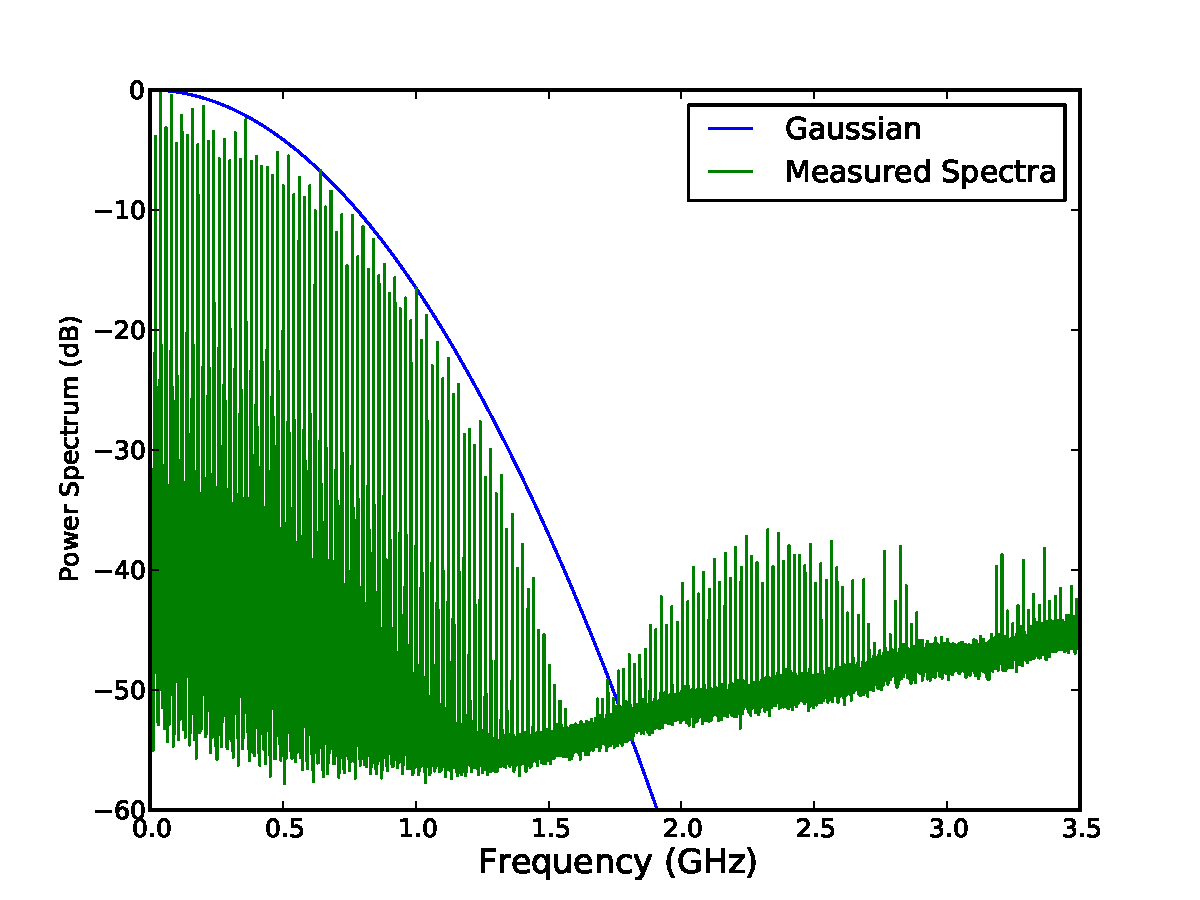
\includegraphics[width=0.45\textwidth]{Wakefields_and_Impedances/figures/beam_spectra_power_gauss_meas_12ns.pdf}
\label{fig:gauss_meas_freq}
}
\subfigure[]{
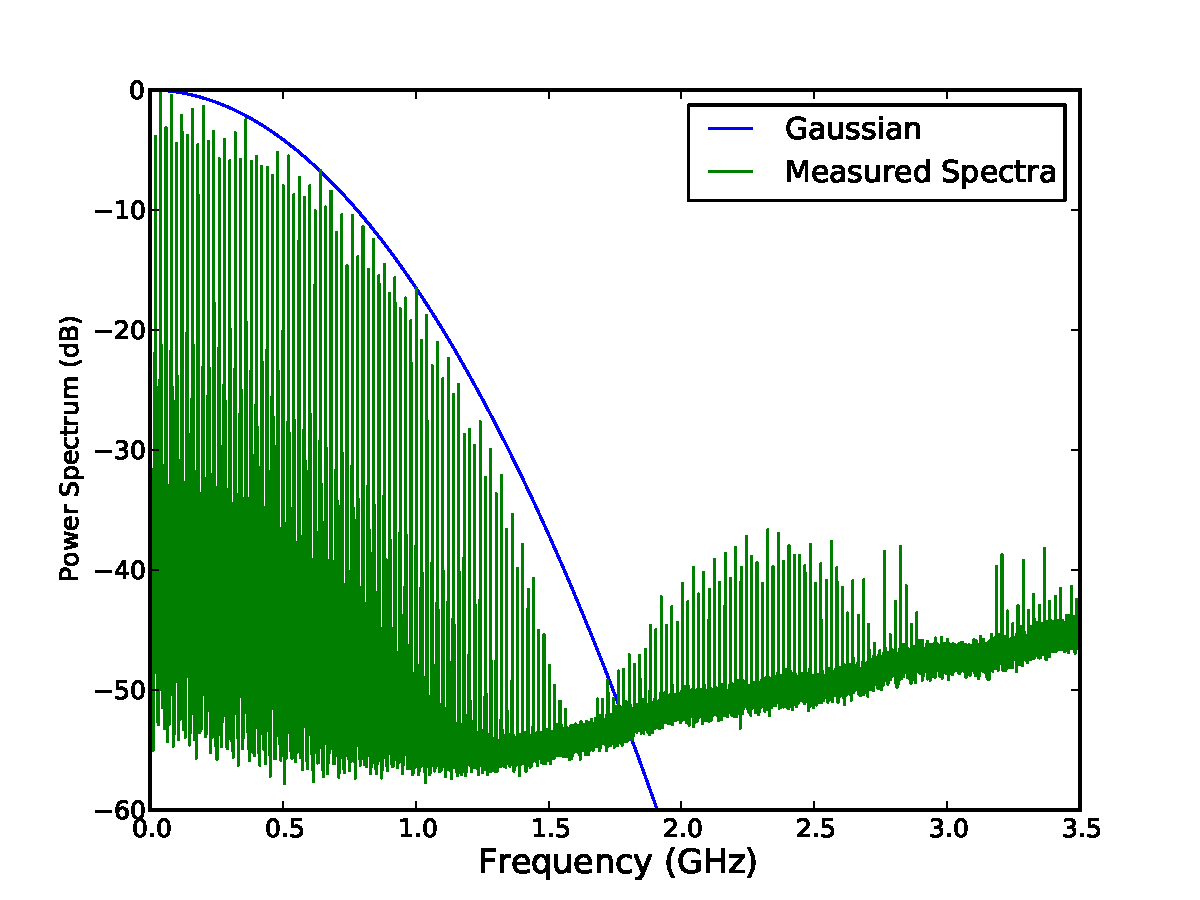
\includegraphics[width=0.45\textwidth]{Wakefields_and_Impedances/figures/beam_spectra_power_gauss_meas_12ns.pdf}
\label{fig:gauss_meas_time}
}
\caption{A comparison of \ref{fig:gauss_meas_freq} a measured beam power spectrum and a Gaussian bunch of the same bunch length in the frequency domain and \ref{fig:gauss_meas_time} the resulting time domain beam profile. The Gaussian has a bunch length (4$\sigma_{z}$ = 1.2ns). Measured spectrum taken by P. Baundrenghien et al \cite{Baudrenghien:LHCPowSpec}.}
\label{fig:measured_gauss}
\end{figure}

As shown by the derivations in Section~\ref{sec:power_loss}, asides from the longitudinal impedance of the device under consideration the longitudinal profile of the circulating bunches also contributes to the power loss in the machine. In past works it has generally been assumed that bunches in accelerators have a Gaussian profile \cite{Grudiev:LongTransSecCol}, given by

\begin{equation}
\lambda \left( t \right) = e^{\frac{-t^{2}}{2\sigma^{2}}}
\label{eqn:gauss}
\end{equation}

where $4\sigma_{z} = t_{b}$ when approaching the analytical treatment of beam induced heating, both single-bunch and multi-bunch. Recent measurements of the power spectrum of particle beams, especially in the LHC \cite{Baudrenghien:LHCPowSpec} have shown characteristics that the Gaussian profile does not predict, for example the high frequency secondary peak as seen in Fig.~\ref{fig:measured_gauss}. To make more realistic predictions of heat loss due to beam impedance in the machine it is thus necessary to find bunch profiles which reproduce this behaviour.

A number of different longitudinal bunch profiles have been investigated in the past. Here we shall look at 3 other bunch profiles; a parabolic line density (see Eqn.~\ref{eqn:para_profile}), cos$^{2}$ (see Eqn.~\ref{eqn:cos_profile}) and a water-bag (see Eqn.~\ref{eqn:water_bag_profile}).

\begin{equation}
\rho\left( t \right) = \int^{\infty}_{-\infty} \lambda \left( \omega \right) e^{j\omega t} d\omega = 
\begin{cases}1-\left( \frac{2t} {t_{b}} \right)^{2} &\textrm{if $| t/2 | \leq t_{b}$}\\
0								&\textrm{if $| t | > t_{b}/2$}
\end{cases}
\label{eqn:para_profile}
\end{equation}

\begin{equation}
\rho\left( t \right) = \int^{\infty}_{-\infty} \lambda \left( \omega \right) e^{j\omega t} d\omega = 
\begin{cases}
cos^{2}\left( \frac{\pi t} {t_{b}} \right) &\textrm{if $| t/2 | \leq t_{b}$}\\
0								&\textrm{if $| t | > t_{b}/2$}
\end{cases}
\label{eqn:cos_profile}
\end{equation}

\begin{equation}
\rho\left( t \right) = \int^{\infty}_{-\infty} \lambda \left( \omega \right) e^{j\omega t} d\omega = 
\begin{cases}
\sqrt{1-\left( \frac{2t}{t_{b}}\right)^{2}} &\textrm{if $| t/2 | \leq t_{b}$}\\
0								&\textrm{if $| t | > t_{b}/2$}
\end{cases}
\label{eqn:water_bag_profile}
\end{equation}

The corresponding frequency domain profiles are given by Eqn.~\ref{eqn:para_profile_freq} for the parabolic profile, Eqn.~\ref{eqn:cos_profile_freq} for the cos$^{2}$ profile, and Eqn.~\ref{eqn:water_bag_profile_freq} for the waterbag profile,

\begin{equation}
 \lambda \left( f \right) = 
\label{eqn:para_profile_freq}
\end{equation}

\begin{equation}
\lambda \left( f \right)  = \frac{sin \left( \pi f t_{b} \right)}{\pi f t_{b} \left[ 1 - \left( f t_{b} \right) \right]}
\label{eqn:cos_profile_freq}
\end{equation}

\begin{equation}
\lambda \left( f \right) = 
\label{eqn:water_bag_profile_freq}
\end{equation}

\begin{figure}
\begin{center}
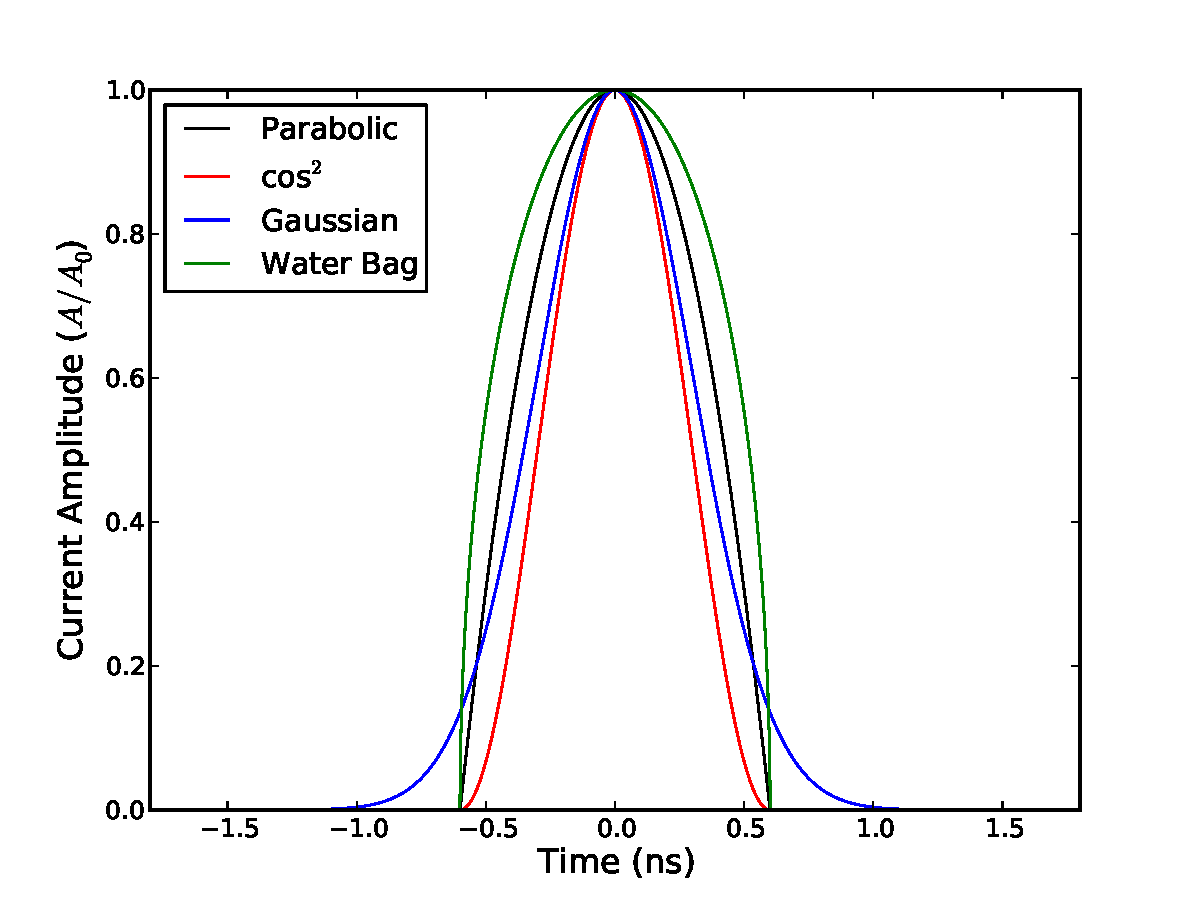
\includegraphics[width=0.65\textwidth]{Wakefields_and_Impedances/figures/bunch_profile_12ns.pdf}
\end{center}
\label{fig:time_bunch_profiles}
\caption{The longitudinal bunch profile of a number of bunch distributions. Note that all of these are normalised to have a peak bunch current of 1. For the Gaussian distribution the bunch length is the 4$\sigma$ value. The bunch length $\tau_{b} = 1.2ns$}
\end{figure}

\begin{figure}
\subfigure[]{
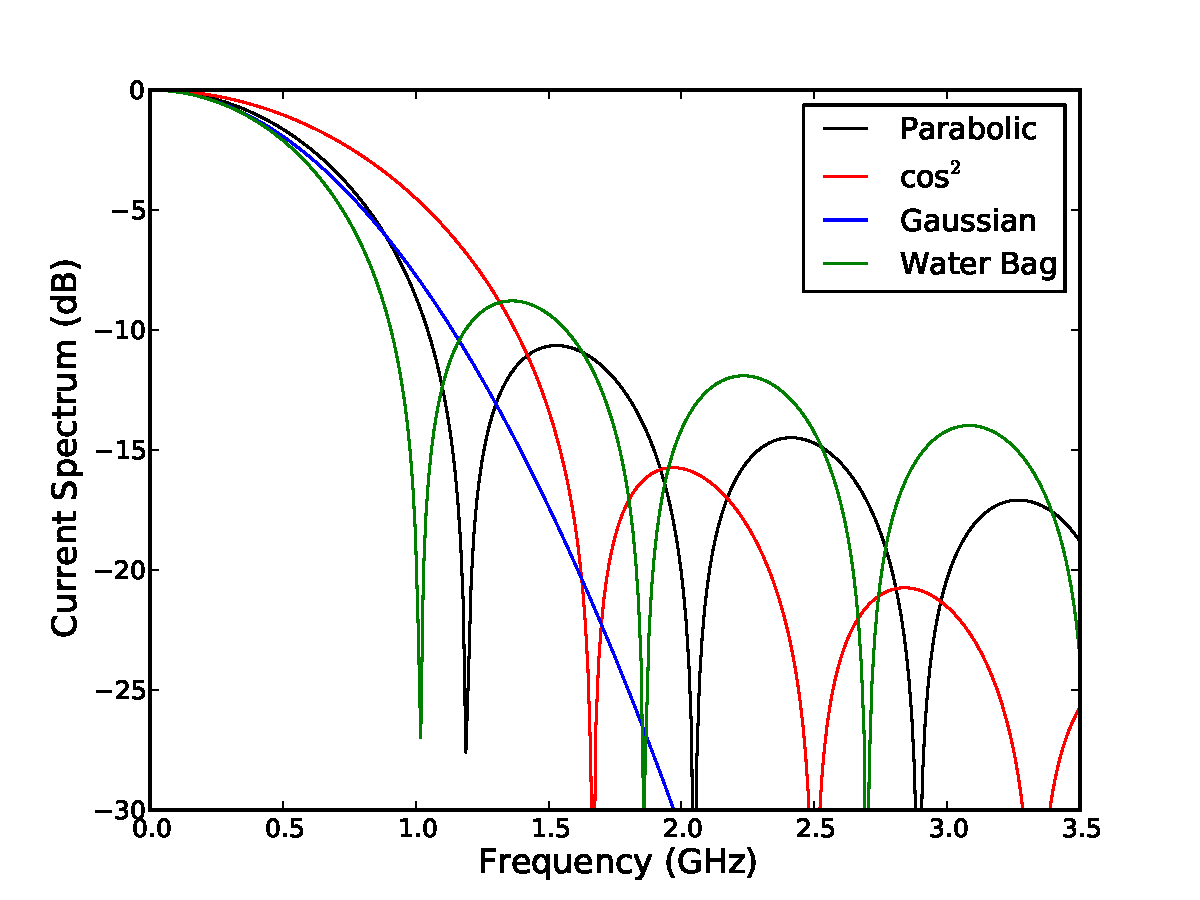
\includegraphics[width=0.45\textwidth]{Wakefields_and_Impedances/figures/current_spectrum_12ns.pdf}
\label{fig:current_spec}
}
\subfigure[]{
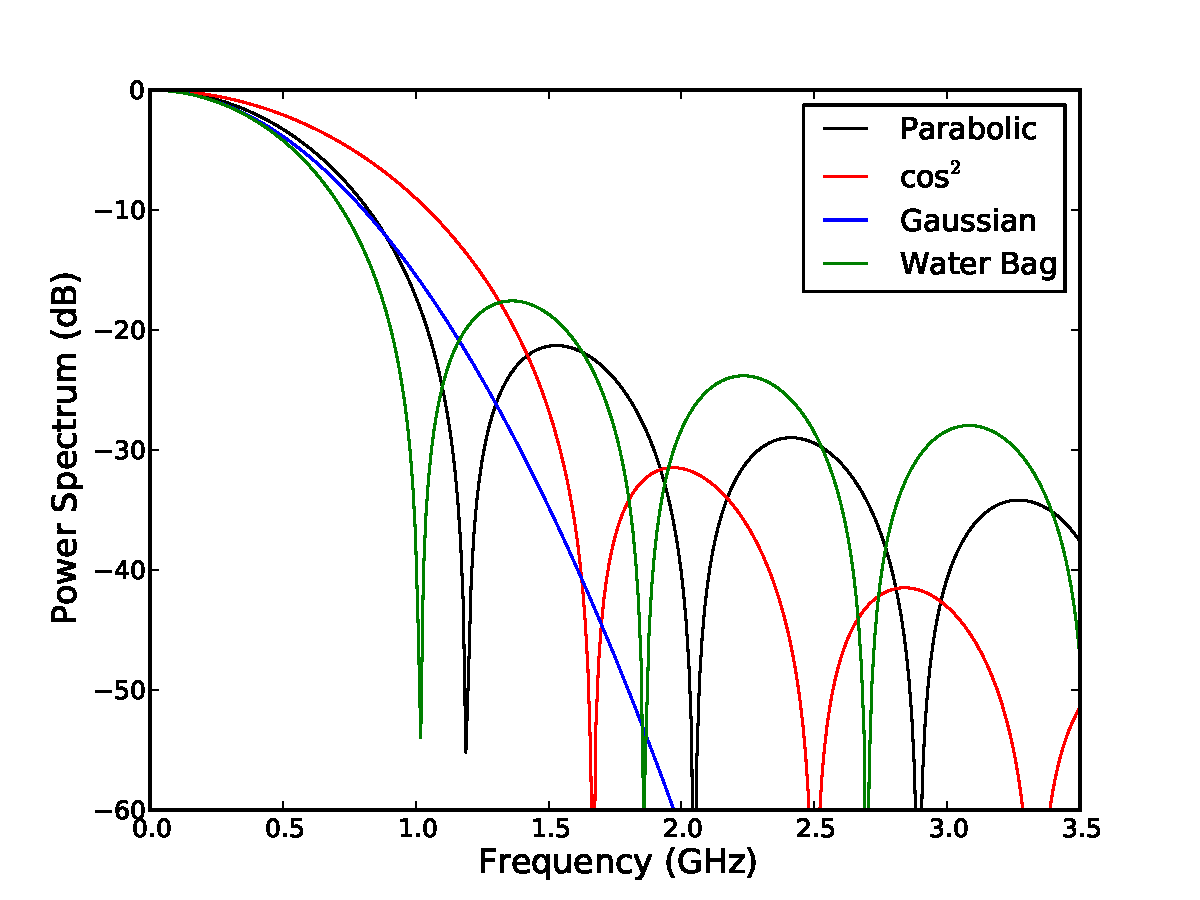
\includegraphics[width=0.45\textwidth]{Wakefields_and_Impedances/figures/power_spectrum_12ns.pdf}
\label{fig:power_spec}
}
\caption{The frequency domain \ref{fig:current_spec} current spectrum and \ref{fig:power_spec} power spectrum for a number of different bunch profiles with a bunch length $\tau_{b} = 1.2ns$.}
\label{fig:freq_dom_prof}
\end{figure}

The comparison of these bunch profiles in the time domain are shown in Fig.~\ref{fig:time_bunch_profiles}. Note all bunch currents are normalised to their peak value. The corresponding current and power spectrums are shown in Fig.~\ref{fig:freq_dom_prof}. There are several things to note about these spectra; firstly that the non-infinite distribution of the non-Gaussian bunch profiles gives rise to a number of high frequency lobes in the power spectrum, and secondly the interval of these nodes depends heavily on the bunch profile.

\begin{figure}
\subfigure[]{
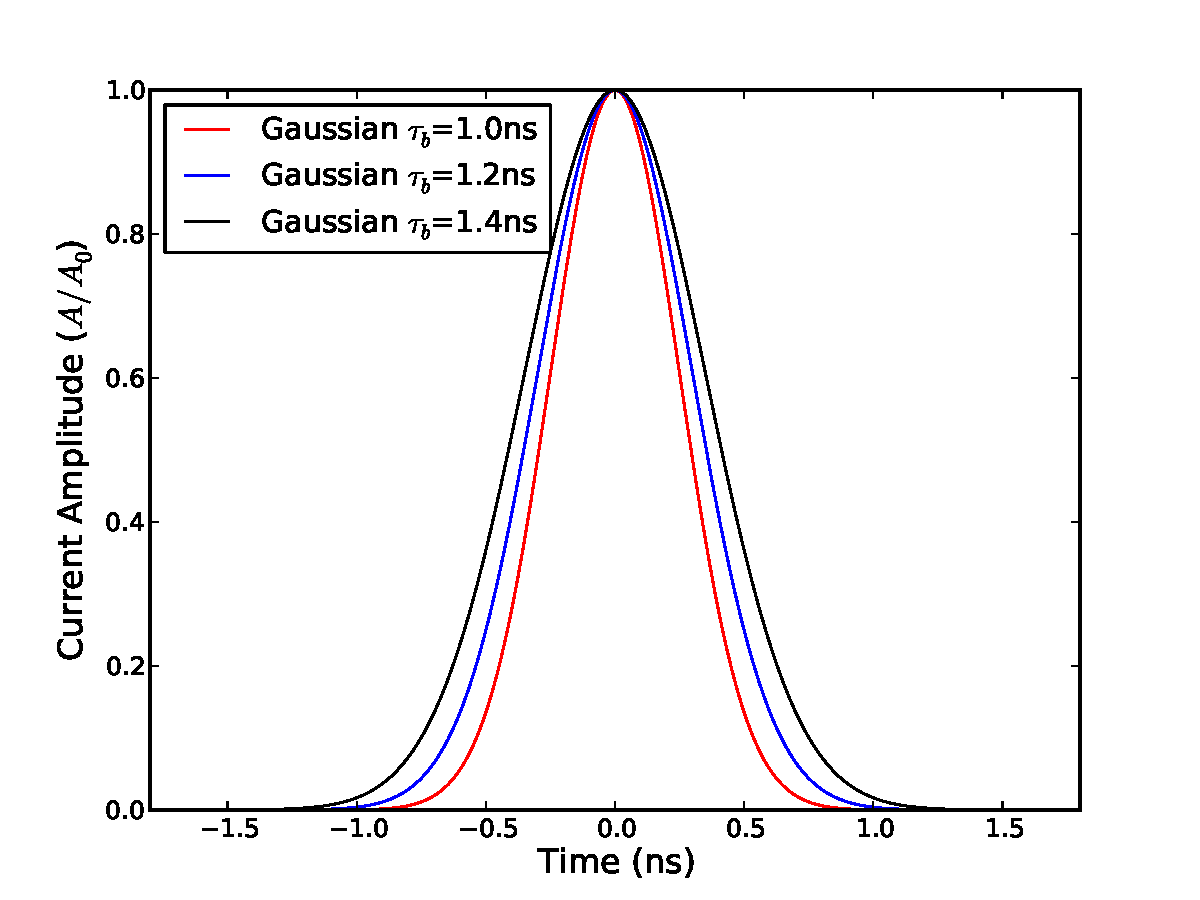
\includegraphics[width=0.45\textwidth]{Wakefields_and_Impedances/figures/gaussian_time_dom_diff_lengths.pdf}
\label{fig:change_len_time_gauss}
}
\subfigure[]{
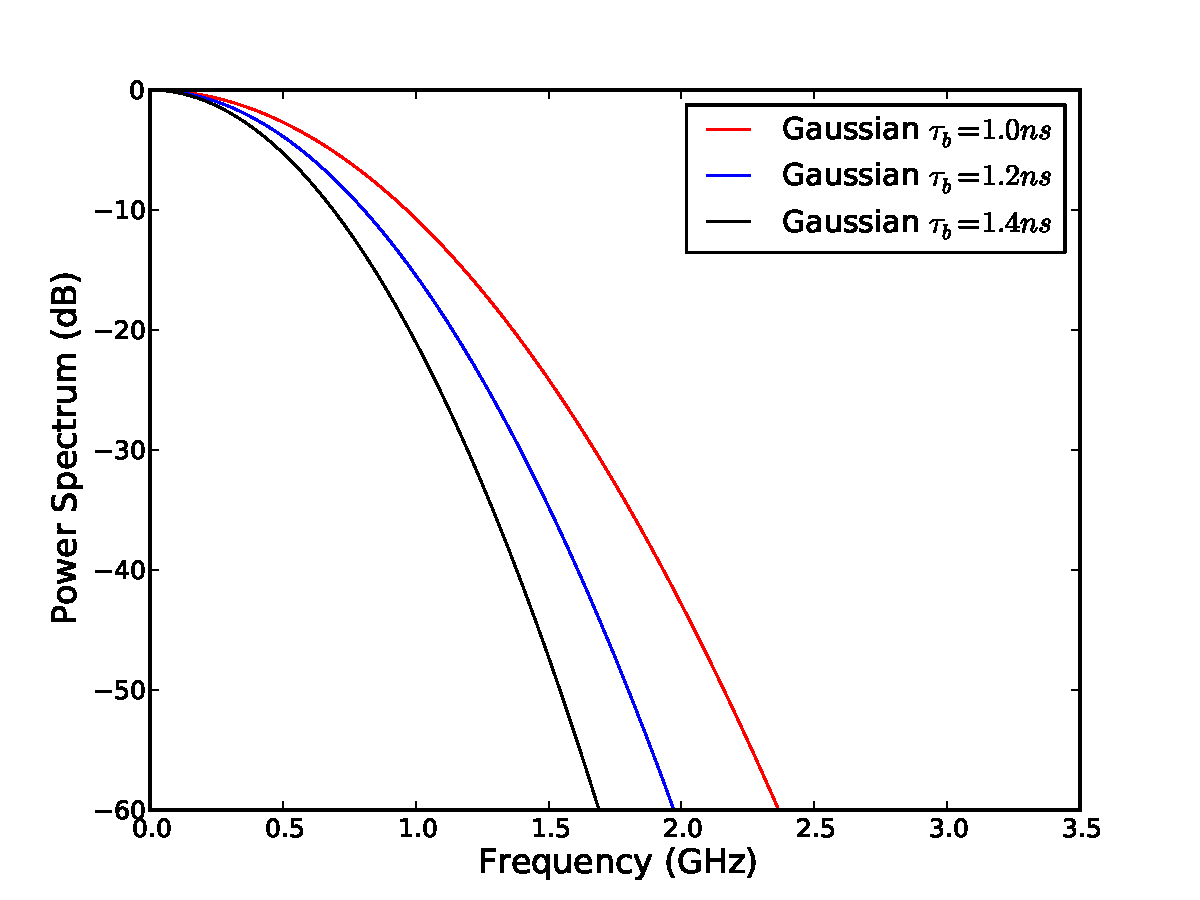
\includegraphics[width=0.45\textwidth]{Wakefields_and_Impedances/figures/gaussian_power_spec_diff_lengths.pdf}
\label{fig:change_len_freq_gauss}
}
\caption{\ref{fig:change_len_time_gauss} The longitudinal profile and the \ref{fig:change_len_freq_gauss} associated bunch power spectrum for a number of bunch lengths assuming a Gaussian bunch profile.}
\label{fig:diff_bunch_len_gauss}
\end{figure}

\begin{figure}
\subfigure[]{
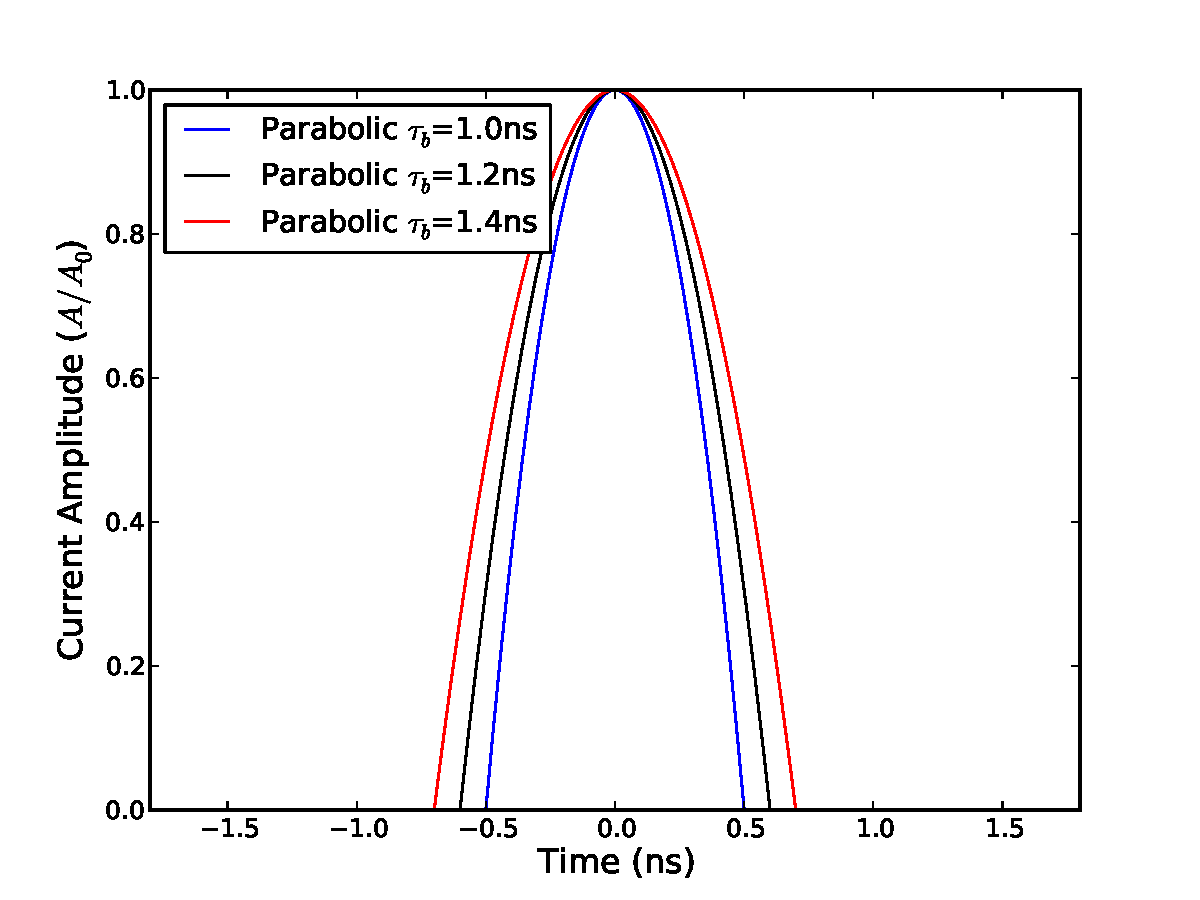
\includegraphics[width=0.45\textwidth]{Wakefields_and_Impedances/figures/current_amp_para_change.pdf}
\label{fig:change_len_time_para}
}
\subfigure[]{
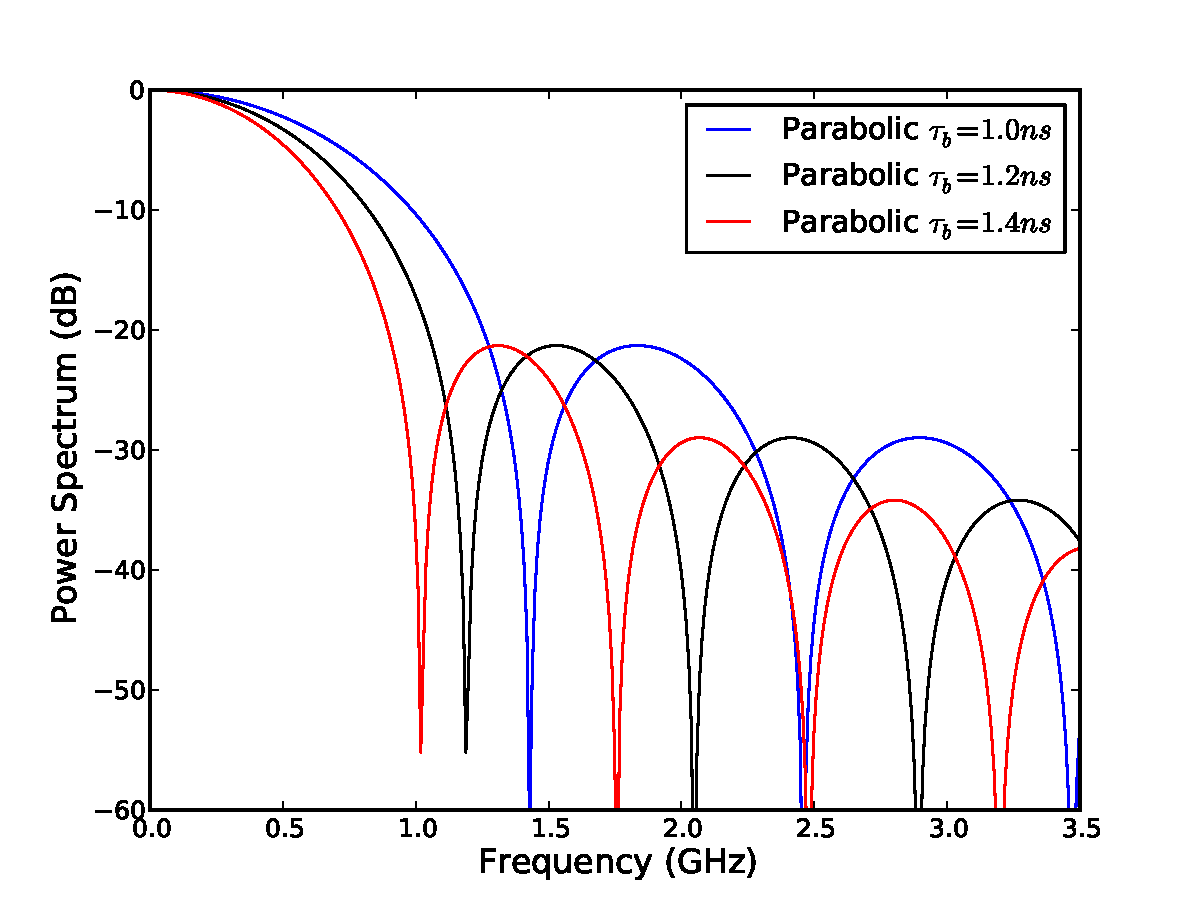
\includegraphics[width=0.45\textwidth]{Wakefields_and_Impedances/figures/freq_power_para_change.pdf}
\label{fig:change_len_freq_para}
}
\caption{\ref{fig:change_len_time_para} The longitudinal profile and the \ref{fig:change_len_freq_para} associated bunch power spectrum for a number of bunch lengths assuming a parabolic bunch profile.}
\label{fig:diff_bunch_len_para}
\end{figure}

To illustrate more clearly the effect of changing the bunch length on the power spectrum, a number of bunch profiles and the corresponding power spectra with different bunch lengths are shown in Fig~\ref{fig:diff_bunch_len_gauss}. Firstly, consider a Gaussian bunch profile. It can be seen in Fig.~\ref{fig:diff_bunch_len_gauss} that by increasing the bunch length that the magnitude at high frequencies is decreased quite substantially. If we consider a finite bunch profile (non-Gaussian), we note that we have high frequency lobes. The peak frequency of these lobes depends on the bunch length, as illustrated using a parabolic bunch profile for bunch lengths $\tau_{b} = 1ns, 1.2ns, 1.4ns$ in Fig.~\ref{fig:diff_bunch_len_para}. As the bunch length is increased the lobes move to lower frequencies, and the width of the first branch decreases. Similar behaviour is observed with the cos$^{2}$ and water-bag bunch profiles.

\begin{figure}
\begin{center}
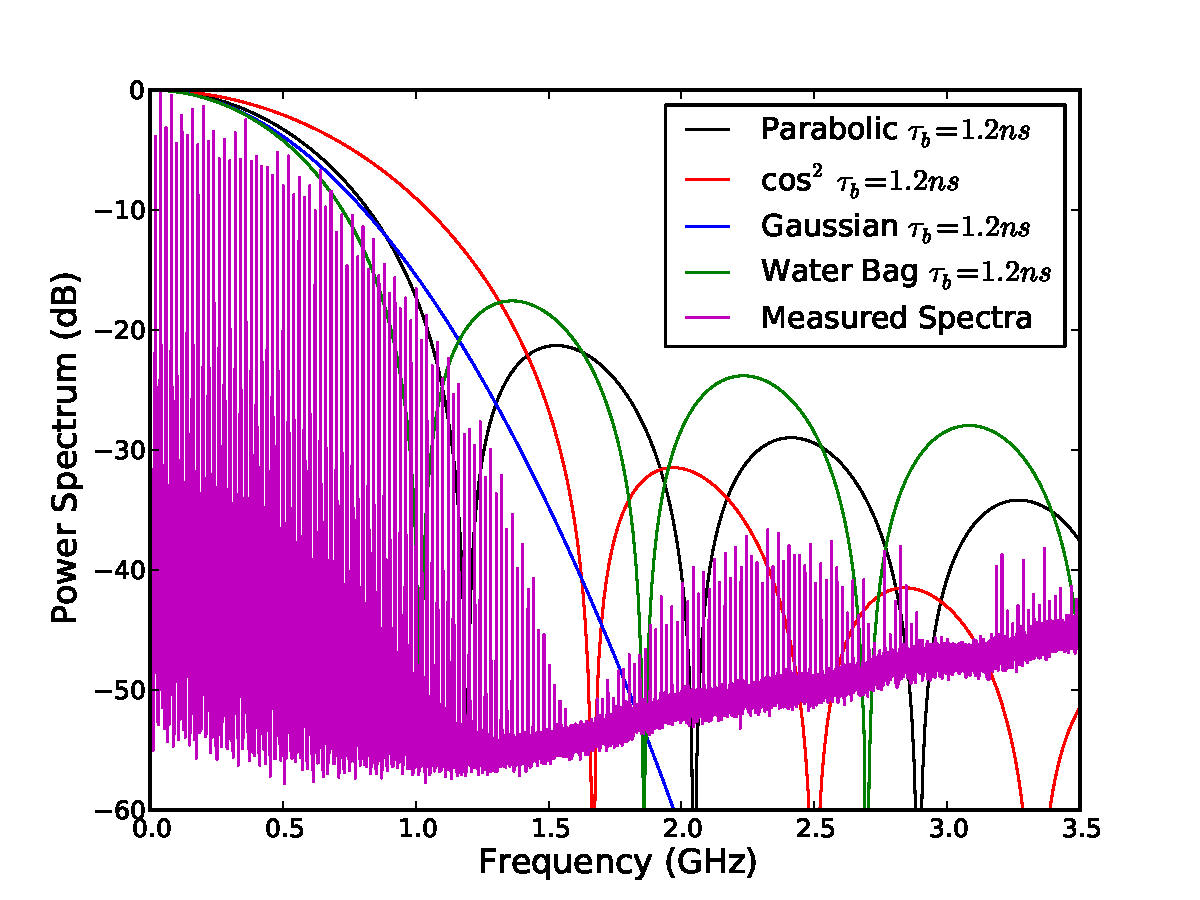
\includegraphics[width=0.65\textwidth]{Wakefields_and_Impedances/figures/beam_spectra_power_12ns.pdf}
\end{center}
\caption{A comparison of a measured beam power spectrum and a number of analytical bunch profiles assuming a bunch length of 1.2ns.}
\label{fig:power_all}
\end{figure}

Finally, a comparison of a measured bunch power spectra and the analytical power spectra is shown in Fig.~\ref{fig:power_all}. It can be seen that whilst it is possible to replicate some of the properties of the measured spectrum, an exact replication is non-trivial. Further investigation into the appropriate bunch profile is ongoing.



% Introduce a number of longitudinal profiles in time domain - gaussian, parabolic line density, cos^2, water bag - comments of realism (gaussian being infinite) - truncated gaussian
% Comparison in the frequency domain - firstly gaussian compared to truncated gaussian - infinite tails reduce the magnitude of the higher frequency components and lobe
% Gaussian, parabolic, cos^2 - all with the same bunch length
% Using the above examples try using a number of different bunch lengths to illustrate how they change (gaussian - just extends further, parabolic, cos^2 lobe frequency changes)
% Finally - comparison to measured spectra to illustrate changes in bunch length and frequency components as bunch is ramped and squeezed

\subsubsection{Beam induced heating due to a low Q impedance}

For an impedance with a characteristic Q that is small (Q $<$ 10), it can be seen that the impedance peak will interact substantially with a number of beam harmonics (see Fig.~\ref{fig:low_q_harmonics}) due to the broad frequency range it occupies.

\begin{figure}
\begin{center}
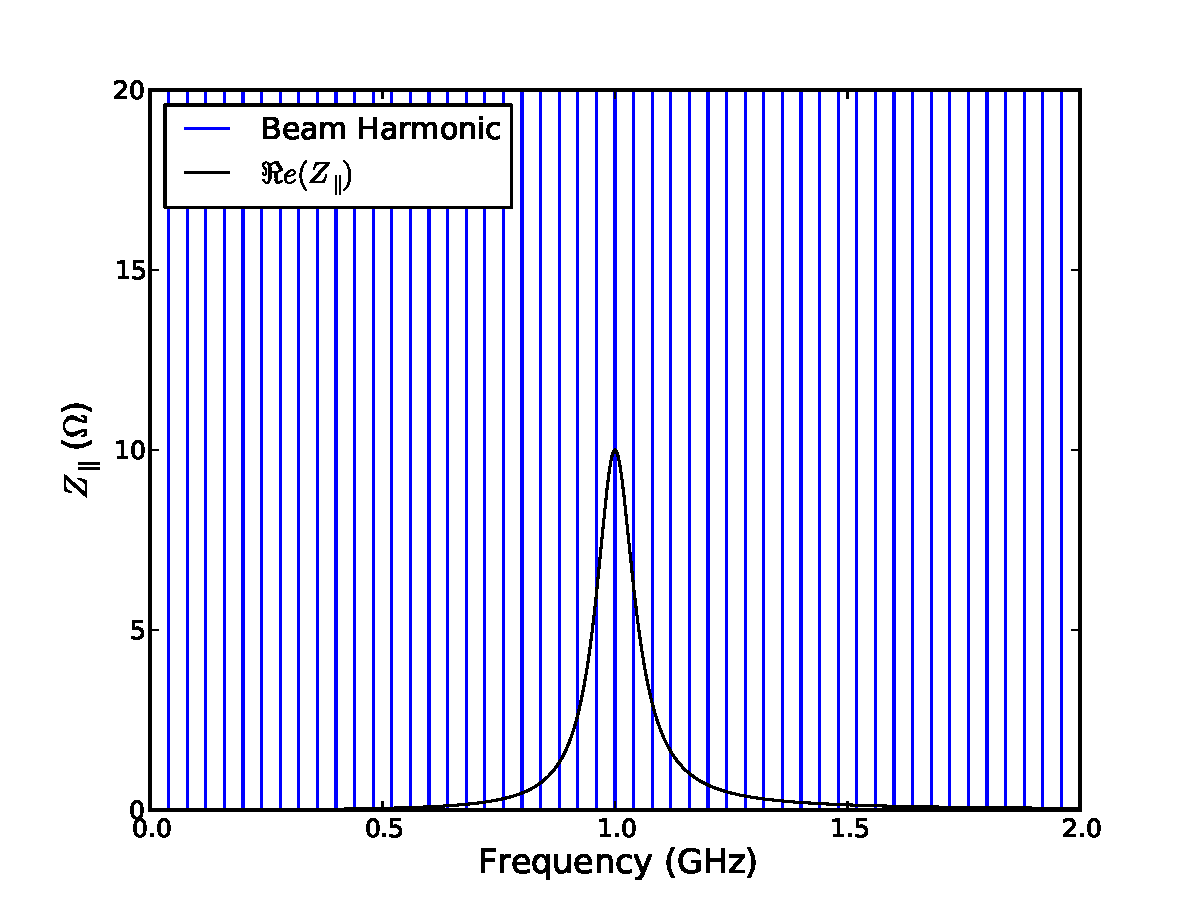
\includegraphics[width=0.65\textwidth]{Wakefields_and_Impedances/figures/low_q_10_resonance_beam_harmonics.pdf}
\end{center}
\caption{The beam harmonics of a beam with a bunch spacing of 25ns overlayed on the real component of the longitudinal impedance an example of a low Q impedance ($R_{s}=10\omega$, Q = 10, $f_{res}=1GHz$). The blue lines represent the frequency of a beam harmonic, not necessarily the magnitude of the power spectrum at that point. Note that a number of beam harmonics overlay non-zero impedance values.}
\label{fig:low_q_harmonics}
\end{figure}

Further investigation of the longitudinal beam spectrum reveals that there is significant structure between the major harmonics (which are due to the bunch spacing of the beam) which can be attributed to the other time structures of the beam, for example the bunch train spacing, or the interval between the pilot bunch train and the subsequent bunch train. As such the treatment of the estimation of beam losses requires a broad spectrum approach. If we consider Eqn.~\ref{eqn:heating-gen} we see that we can treat the power losses in an integral form. We can observe a number of properties using this assumption. The power loss is proportional to the beam properties in the following manner:

\begin{enumerate}
\item{$P_{loss} \propto N^{2}$}
\item{$P_{loss} \propto n_{bunch}$}
\end{enumerate}

\subsubsection{Beam induced heating due to a high Q impedance}

In contrast to the overlap of the beam spectrum with a low Q impedance, for a high Q impedance only one beam harmonic lies upon the resulting impedance to any significant quantity. This is illustrated in Fig~\ref{fig:high_q_harmonics}. If we consider Eqn \ref{eqn:heating-gen} and consider the situation where

\begin{equation}
\left( 2 \left| \lambda \left(p \omega_{rev}n_{bunch} \right)  \right|^{2}  \Re{}e \left( Z_{\parallel} \left(p \omega_{rev}n_{bunch}\right) \right) \right) = 
\begin{cases}
\left( 2 \left| \lambda \left( \omega_{res} \right)  \right|^{2}  \Re{}e \left( Z_{\parallel} \left( \omega_{res} \right) \right) \right) &\textrm{if $p \omega_{rev} n_{bunch} = \omega_{res}$}\\
0								&\textrm{if $p \omega_{rev} n_{bunch} != \omega_{res}$}
\end{cases}
\label{eqn:single_harmonic_profile}.
\end{equation}

\begin{figure}
\begin{center}
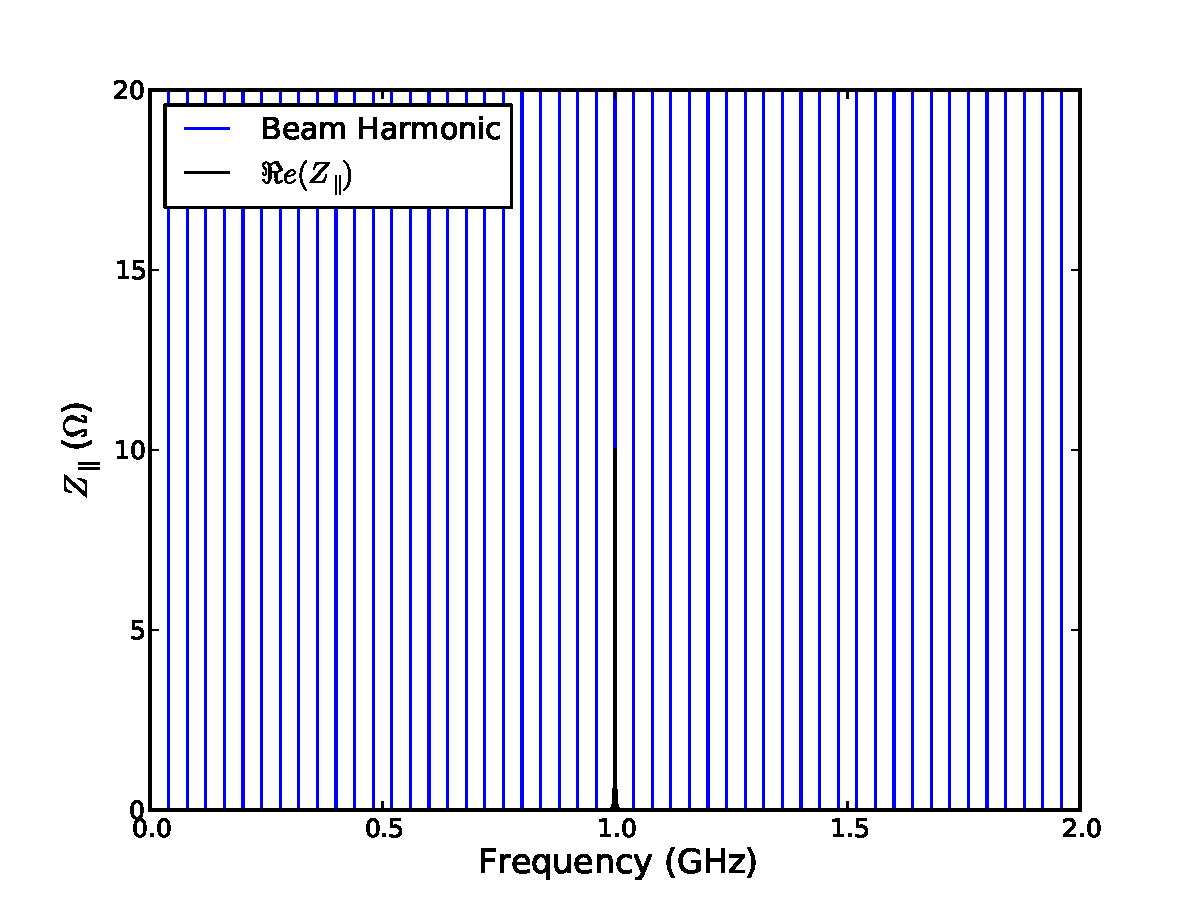
\includegraphics[width=0.65\textwidth]{Wakefields_and_Impedances/figures/high_q_1000_resonance_beam_harmonics.pdf}
\end{center}
\caption{The beam harmonics of a beam with a bunch spacing of 25ns overlayed on the real component of the longitudinal impedance of a sample of a high Q impedance ($R_{s}=10\Omega$, Q = 1000, $f_{res}=1GHz$). The blue lines represent the frequency of a beam harmonic, not necessarily the magnitude of the power spectrum at that point. Note that only a single beam harmonic overlays a non-zero impedance values.}
\label{fig:high_q_harmonics}
\end{figure}

It can then be seen that Eqn~\ref{eqn:heating-gen} simplifies to

\begin{equation}
P_{loss} = \left( \omega_{rev}eN_{b}n_{bunch}  \right)^{2}  \left( 2 \left| \lambda \left( \omega_{res} \right)  \right|^{2}  \Re{}e \left( Z_{\parallel} \left(\omega_{res} \right) \right) \right). 
\label{eqn:heating-high-q}
\end{equation}

The following properties can subsequently be seen as a result:

\begin{enumerate}
\item{$P_{loss} \propto N^{2}$}
\item{$P_{loss} \propto n_{bunch}^{2}$, provided that the resonant frequency of the resonance continues to coincide with a beam harmonic.}
\end{enumerate}

\subsubsection{Some Examples of the Beam-Induced Heating}

In this section we shall illustrate some important factors that have been covered in previous sections. In particular, the interaction of different bunch profiles at different bunch lengths with an example cavity resonance will be covered in some detail to illustrate how the estimated heating can change drastically depending on higher frequency lobes in the beam current spectrum. In addition, the heating due to two particle beams in the same vacuum chamber shall be briefly covered for interest.

\subsubsection{The Effect of Bunch Length on Power Loss}

As can be seen in Figs.~\ref{fig:freq_dom_prof} and Fig~\ref{fig:diff_bunch_len_para}, the bunch profile and the bunch length can significantly alter the magnitude of the beam current at higher frequencies. To illustrate this, let us consider two resonant impedances, one broadband $Z_{bb}$ and one narrow band $Z_{nb}$ impedance, characterised by having a low-$Q$ and a high-$Q$ respectively. Both impedances shall have the same resonant shunt impedance $R_{s} = 100\Omega$. The broadband impedance shall have a $Q_{bb}=1$, and the narrow band impedance $Q_{nb}=1000$. The resonant frequency will be changed to illustrate effects in different regimes of the bunch length and of different bunch profiles.

We shall use the Gaussian bunch profile and the $cos^{2}$ bunch profile for these examples. The Gaussian is useful to illustrate the effect of just changing the bunch length, and the $cos^{2}$ due to the presence of a high frequency lobe in it's frequency domain current spectrum. The $cos^{2}$ frequency domain current profile is given by

\begin{equation}
I \left( \omega \right) = \frac{sin \left( \omega \tau_{b}/2 \right)}{ \omega \tau_{b}/2 \left[ 1 - \left(  \omega \tau_{b}/2 \right)^{2}  \right]}.
\end{equation}

\begin{figure}
\begin{center}
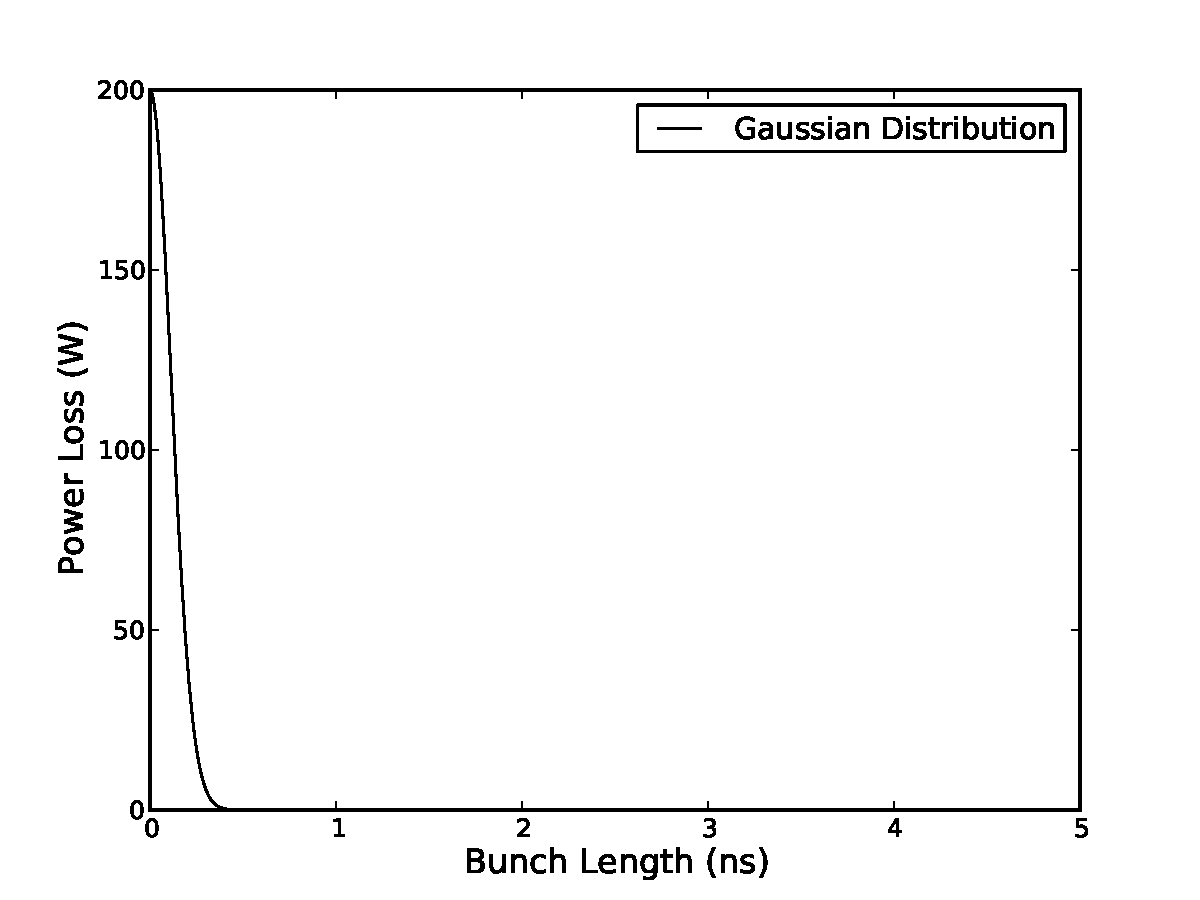
\includegraphics[width=0.8\textwidth]{Wakefields_and_Impedances/figures/heating_narrowband_gauss_bunch_length.pdf}
\end{center}
\caption{The change in power loss due to a narrow band resonance characterised by $\omega_{0} = 2GHz$, $R_{s} = 100\Omega$, $Q = 1000$ with a Gaussian bunch distrbution of different lengths.}
\label{fig:bunch_length_heat_narrow}
\end{figure}

First we shall consider a narrow band impedance which has a resonant frequency $\omega_{0} =2GHz$ which falls upon a beam harmonic such that $\omega_{0}=n\omega_{rev}$, where $n$ is an integer. It should be noted that for other cases the contribution of these sources of heating is negligible due to the small beam current at this frequency. There are two extreme cases; that of  $\omega_{0} \gg 1/\tau_{b}$, in which it can be seen that the current spectrum will be negligible at the frequency of the impedance, and $\omega_{0} \ll 1/\tau_{b}$ where the beam current spectrum is essentially the same as the DC spectral component. The transition in this intervening regime is shown in Fig~\ref{fig:bunch_length_heat_narrow}, assuming a bunch current of 1A. It can be seen that in this case the heating falls drastically as the bunch length increases.

If we instead consider a cos$^{2}$ distribution we instead see the effect of the secondary lobes in the beam current spectrum. The power loss with bunch length is shown in Fig.~\ref{fig:bunch_length_heat_narrow} in comparison to that of the Gaussian profile. The beam power spectrum for a number of different bunch lengths are shown with the real component of the longitudinal impedance in Fig.~\ref{fig:imp_profile_cos}. Here it can be clearly seen that the intersection of the secondary lobe with the resonant impedance causes a peak in the power lost by the beam, highlighting the neccessity to be aware of the frequencies of resonant impedances with relation to the beam harmonics.


\begin{figure}
\subfigure[]{
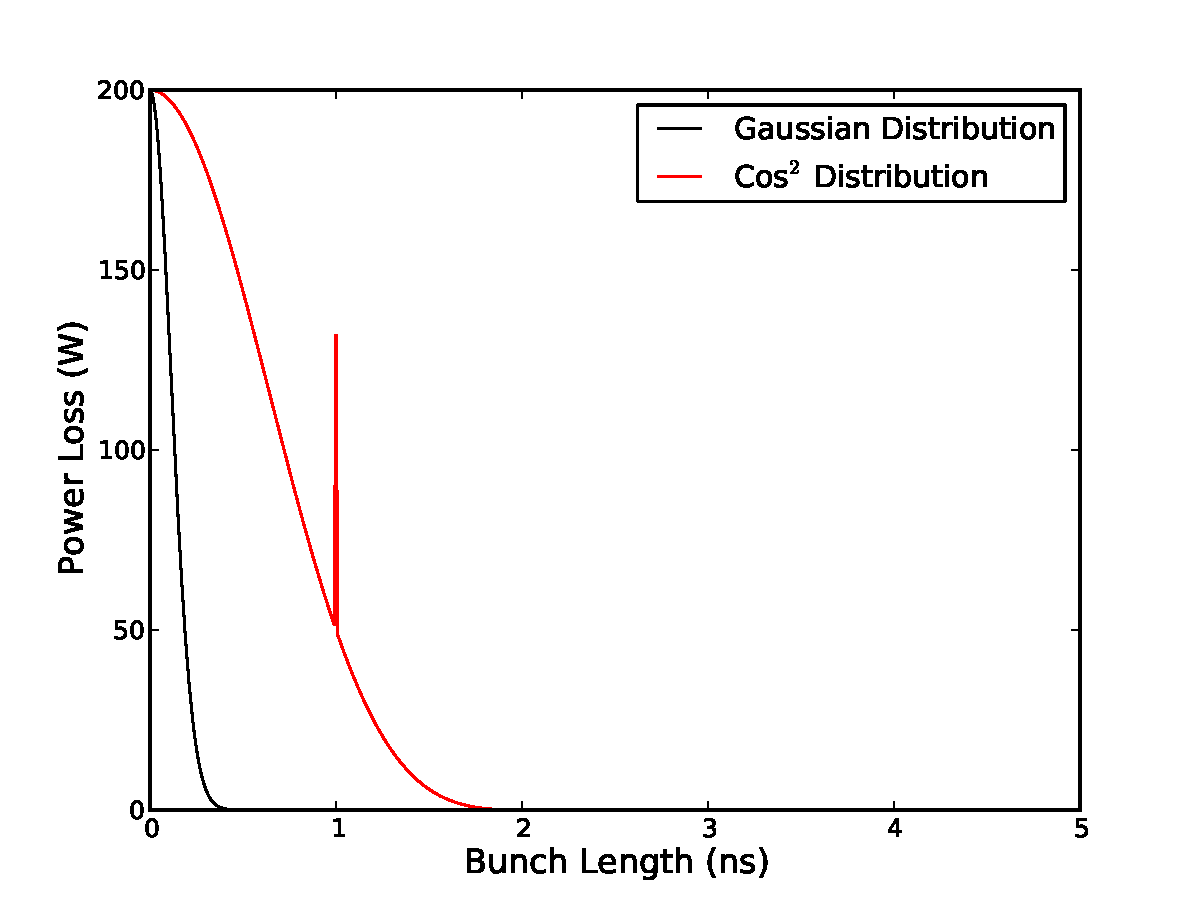
\includegraphics[width=0.5\textwidth]{Wakefields_and_Impedances/figures/heating_narrowband_gausscos_bunch_length.pdf}
\label{fig:long_imp_narrow_current}
}
\subfigure[]{
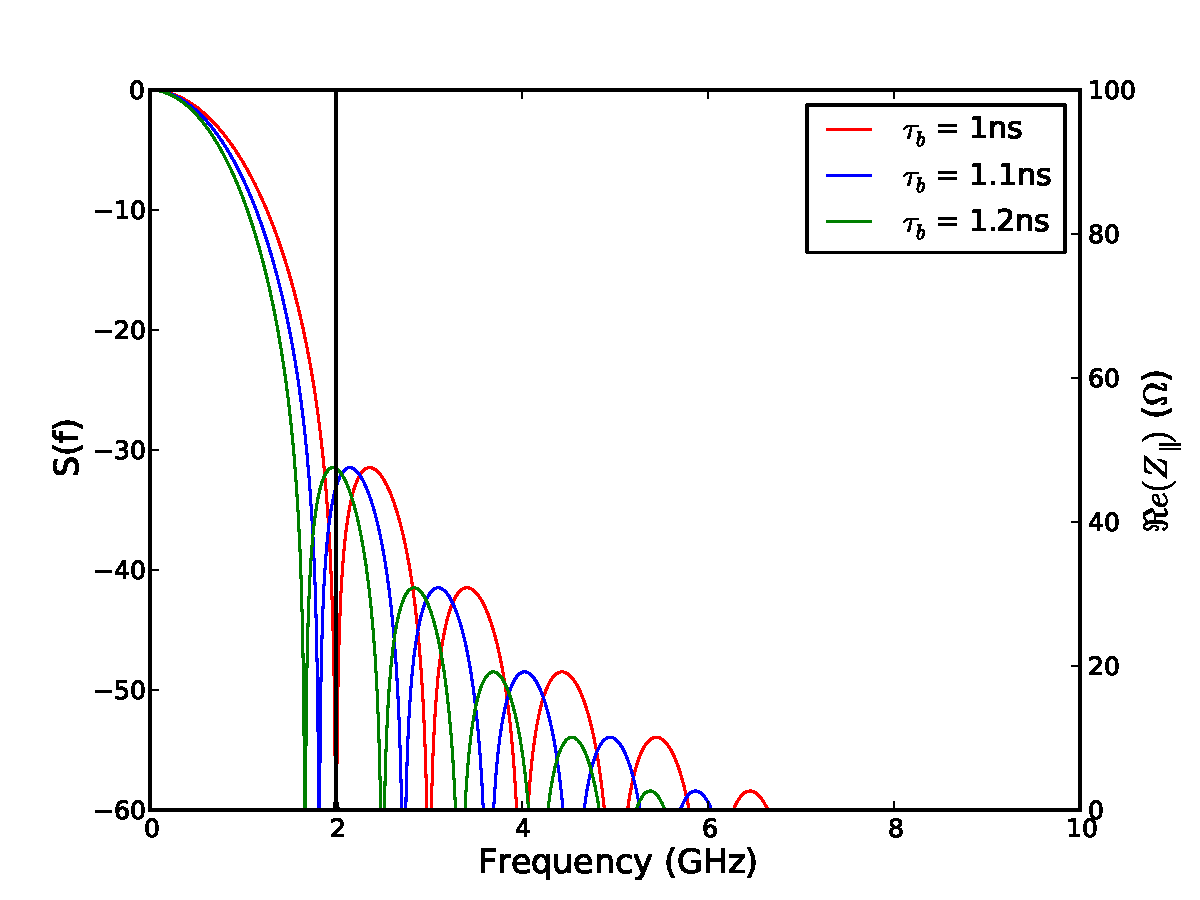
\includegraphics[width=0.5\textwidth]{Wakefields_and_Impedances/figures/impedance_and_power_cos_res.pdf}
\label{fig:imp_profile_cos}
}
\caption{\ref{fig:long_imp_narrow_current} The change in power loss due to a narrow band resonance characterised by $\omega_{0} = 2GHz$, $R_{s} = 100\Omega$, $Q = 1000$ interacting with a cos$^{2}$ bunch distribution with different bunch lengths. The impedance and the beam power spectrum are shown in \ref{fig:imp_profile_cos} to illustrate how this relates to the power loss.}
\end{figure}

\begin{figure}
\subfigure[]{
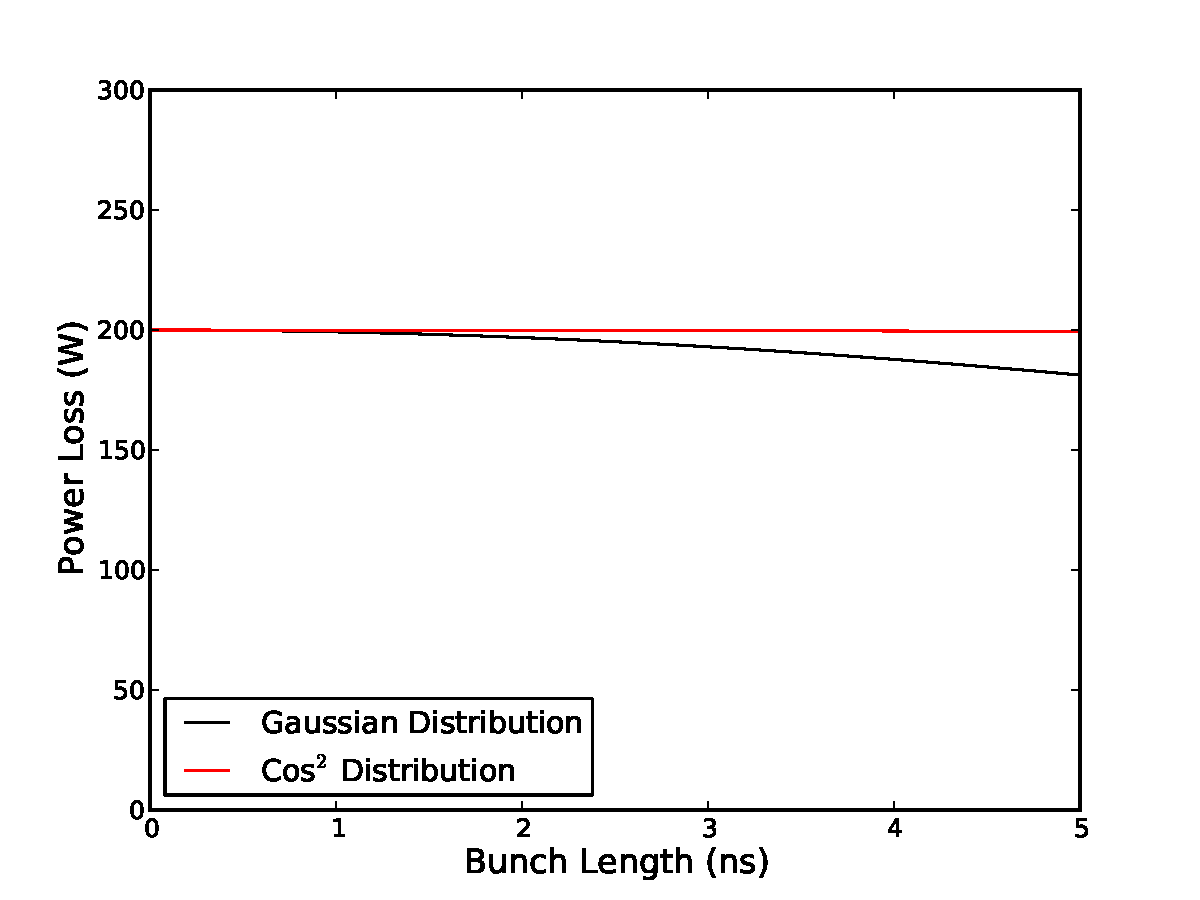
\includegraphics[width=0.5\textwidth]{Wakefields_and_Impedances/figures/heating_broadband_gausscos_bunch_length.pdf}
\label{fig:broadband_heat_bunch_len}
}
\subfigure[]{
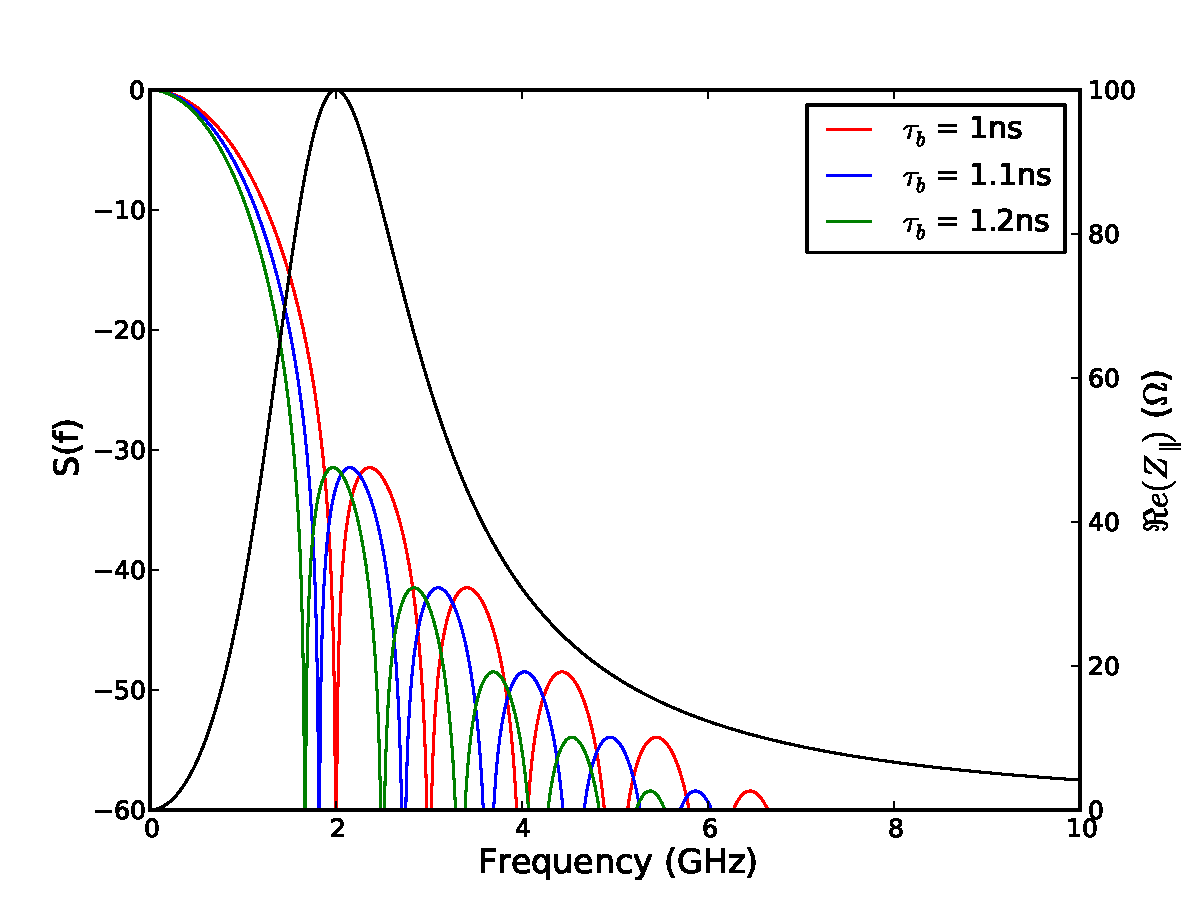
\includegraphics[width=0.5\textwidth]{Wakefields_and_Impedances/figures/impedance_and_power_cos_res_broad.pdf}
\label{fig:broadband_power_loss}
}
\caption{\ref{fig:broadband_heat_bunch_len} The change in power loss due to a narrow band resonance characterised by $\omega_{0} = 2GHz$, $R_{s} = 100\Omega$, $Q = 1$ interacting with a cos$^{2}$ bunch distribution with different bunch lengths. The impedance and the beam power spectrum are shown in \ref{fig:broadband_power_loss} to illustrate how this relates to the power loss.}
\end{figure}


For the broadband heating we shall consider a resonant impedance defined by the following parameters, $\omega_{0} = 2GHz$, $Q=1$, $R_{s}=100\Omega$. To account for the multiple beam harmonics that will interact with the resonance, it is assumed that the beam harmonics in this case occur at $20$MHz intervals. The impedance and the beam power spectrum is shown in Fig.~\ref{fig:broadband_heat_bunch_len} and the resulting power loss in Fig.~\ref{fig:broadband_power_loss} where it can be seen that the power loss decreases slowly with increasing bunch length. This is due to the significant contribution to the power loss at low frequencies, in which the component of the beam power spectrum decreases only marginally due to the decreasing bunch length.

\subsubsection{Beam-Induced Heating due to two traversing beams}

Previous work \cite{Grudiev:twoBeamCol} has investigated the effect of two beams in a vacuum on the beam-induced heating. This is restated here for the sake of completeness.

To begin, consider the two currents $I_{b1} = I_{0}e^{i\phi_{1}}$ and $I_{b1} = -I_{0}e^{i\phi_{2}}$ representing two counter rotating beams. $I_{0}$ represents the beam current, and $\phi_{1/2}$ the phase of beam 1 and beam 2 respectively. Each beam also sees a seperate potential when it traverses the impedance, given by $V_{b1} = \int_{b1} E_{z} e^{i\omega_{0}z/c} dz$ and $V_{b2} = \int_{b2} E_{z} e^{i\omega_{0}z/c} dz$ respectively. By Ohms law it can then be seen that

\begin{equation}
\begin{pmatrix}
V_{b1} \\
V_{b2}
\end{pmatrix}
=
\begin{bmatrix}
Z_{11} & Z_{12} \\
Z_{21} & Z_{22}
\end{bmatrix}
\begin{pmatrix}
I_{b1} \\
I_{b2}
\end{pmatrix}.
\end{equation}

The power loss due to both beams can then be seen to be

\begin{equation}
P_{loss} = \begin{pmatrix}
V_{b1} & V_{b2}
\end{pmatrix}
\begin{pmatrix}
I_{b1} \\
I_{b2}
\end{pmatrix}^{*}.
\end{equation}

In the worst case scenario, the values of the impedance matrix are real, and are equal in value to the peak values of the resonant impedance
\begin{equation}
Z_{11} = 2R^{b1}_{s};\text{    } Z_{22} = 2R^{b2}_{s};\text{    }  Z_{12} = Z_{21} = 2 \sqrt{R^{b1}_{s}R^{b2}_{s}}.
\end{equation}

The power loss then becomes

\begin{equation}
P_{loss} = I_{0}^{2} 2 \left( R_{s}^{b1} +  R_{s}^{b1} - 2\sqrt{R^{b1}_{s}R^{b2}_{s}} cos \left( \delta \phi \right) \right)
\end{equation}

where $\delta \phi = \phi_{1} - \phi_{2}$ is the phase difference between beam 1 and beam 2. This can be found relatively easily by comparing the distance $\delta s$ from a collision IP (location of experiments in the LHC) of the machine. Assuming the beams are ultrarelativistic $\delta \phi = \omega_{rev} 2  \delta s /c$. It can then be seen that the the last term may either reduce or increase the power loss depending on whether $cos\left( \delta \phi \right) = 1$ or $cos\left( \delta \phi \right) = -1$ respectively.

